\begin{exmp}[Lane Change]
	We use a passing scenario as a running example.
	The scenario shows the ego vehicle driving in the right lane of a uni-directional two lane road network. 
	Another car is driving in front of the ego vehicle at a lower speed.
	The ego vehicle's planner decides to initiate a passing maneuver, which involves moving to the left lane, accelerating to pass the other vehicle, and ending at an intersection to make a left turn.
	See Fig.\ref{fig:scenario}.	
	\begin{figure}[tb]
		\label{fig:scenario}
		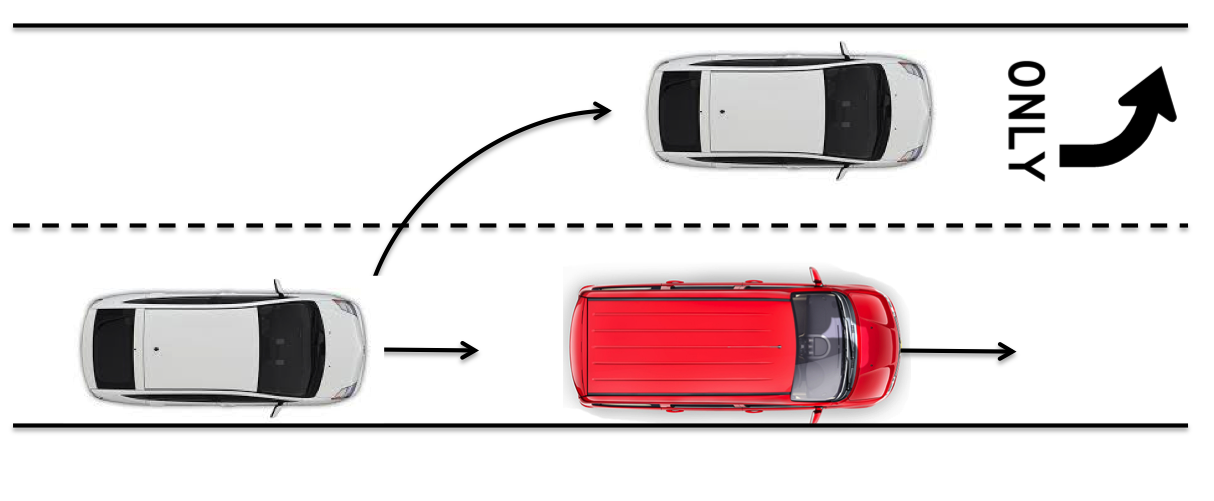
\includegraphics[scale=.4]{scenario.png}
		\caption{Pictorial description of target vehicle scenario}
	\end{figure}
	The safety requirement is that the ego vehicle must remain at least a certain distance away from the other vehicle.
	The mission goal is to arrive and make a right turn at the intersection.
	The verification engineer is given a vehicle controller and must check formally that the closed-loop system (ego vehicle + controller) performs correctly and safely: the ego vehicle
	\begin{enumerate}
		\item may not exceed the speed limit (safety).
		\item may not collide with any other vehicles (if they exist) on the road (safety).
		\item must stop at a red light (safety).
		\item must eventually complete the scenario (liveness).
	\end{enumerate}
	Ideally, the closed-loop system can be formally verified, which requires dynamics that are simple enough to be decidable and within reach of available model checkers.
	Yet the safety requirement requires us to work with the accurate dynamics to determine the cars' movements during a lane change, especially during lateral changes of position. 
	Thus we need both model checking techniques, and reachability computations, to verify the safe and correct completion of this sequence of scenarios.
	The `handing over' from one formalism/scenario to the next formalism/scenario must be correct.
\end{exmp}

\begin{exmp}[Lane change continued]
	The mission can be decomposed into the following scenarios:
	$M = $ DriveStraight, ChangeLane, PassOnTheLeft, StopAtFourWayIntersection.
	Each of these scenarios contains two instances $v_{ego}$ and $v_2$ of the \texttt{vehicle} agent type, one \texttt{road} agent instance, no \texttt{pedestrian}s and one \texttt{trafficSignage} agent.
	The behavior $\behavior_{v_2}$ is given by a sequence of reach sets as detailed in Section \ref{otherAgents};
	briefly, $\behavior_{v_2}$ gives the area occupied by $v_2$ at any moment in time.
	An example applicable law, expressed in discrete time LTL, is $l \defeq \always(position_{ego} = a \implies X position_{ego} \geq a)$, to indicate that backing up is not allowed.
	Note that LTL is not ideally suited for this requirement since we need one formula per speed threshold $a$. A more concise logic (e.g., TPTL \cite{alur94_really}) would allow us to directly say $l \defeq \always(position_{ego}(t+1) \geq position_{ego}(t))$, while still being reasonably computationally tractable.
		
	There are two exit conditions for the DriveStraight scenario: either the ego vehicle reaches the end of the current road segment (i.e. , it reaches the intersection). 
	Or, it gets too close to the leading vehicle $v_2$, in which case it must exit and scenario ChangeLane begins.
	The $Init$ set for ChangeLane is the union of two sets $Init_1$ and $Init_2$.
	$Init_1$ is the set of 2D positions on the road where $v_ego$ is behind $v_2$ and within some distance $d_{min}$ of $v_2$.
	$Init_2$ is the set of 2D positions of $v_{ego}$ that are some distance $d_{turn}$-close to the intersection.
	I.e., we consider the lane change to be provoked by excessive proximity to the leading vehicle $v_2$, or by proximity to the intersection.	
\end{exmp}